\section{Einphasige Brückenschaltung - Gesteuerter Betrieb}

\subsection{Messschaltung}

\begin{figure}[h!]
    \centering
    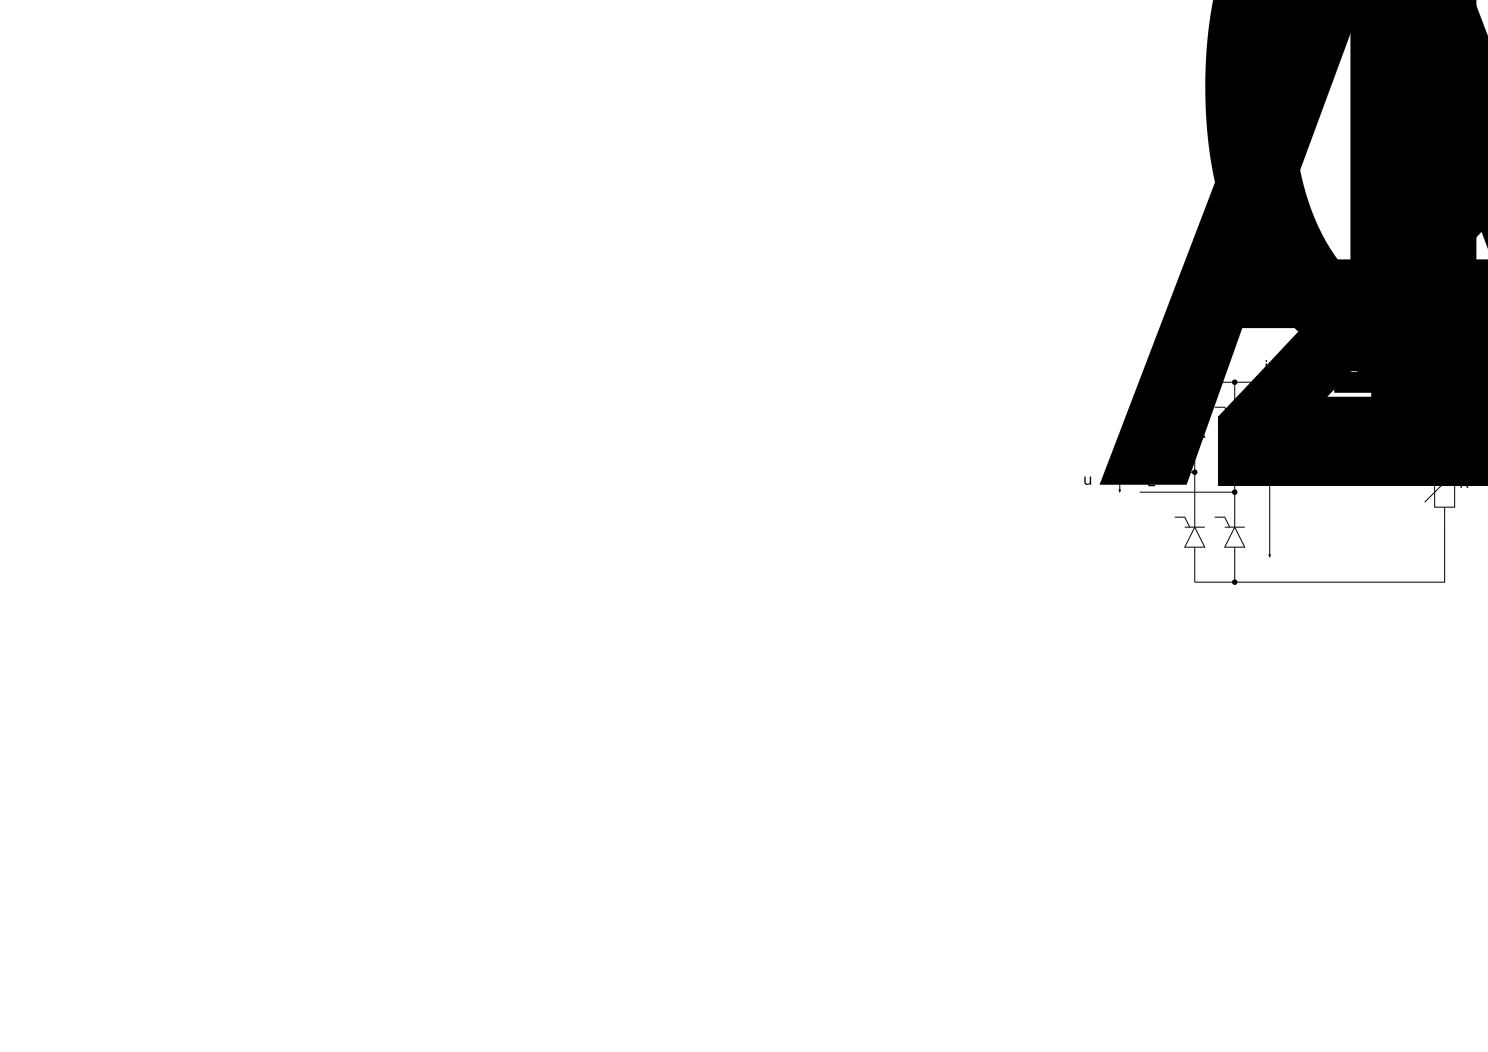
\includegraphics[scale=\sscale]{./../fig/b2_thyristor.pdf}
    \caption{B2 Thyristorgleichichter}
    \label{fig:b2_tyristor}
\end{figure}

\subsection{Messungen}

\begin{figure}[h!]
    \centering
    \includegraphics[scale=\pscale]{./../plots/632_01.pdf}
    \caption{B2 Thyristorgleichrichter mit L-Glättung, Zündwinkel $\alpha$ = 0°}
\end{figure}

\begin{figure}[h!]
    \centering
    \includegraphics[scale=\pscale]{./../plots/632_02.pdf}
    \caption{B2 Thyristorgleichrichter mit L-Glättung, Betrieb an Lückgrenze}
\end{figure}

\begin{figure}[h!]
    \centering
    \includegraphics[scale=\pscale]{./../plots/632_03.pdf}
    \caption{B2 Thyristorgleichrichter mit L-Glättung, lückender Betrieb}
\end{figure}

\begin{figure}[h!]
    \centering
    \includegraphics[scale=\pscale]{./../plots/632_04.pdf}
    \caption{B2 Thyristorgleichrichter mit L-Glättung, lückender Betrieb}
\end{figure}

\begin{figure}[h!]
    \centering
    \includegraphics[scale=\pscale]{./../plots/632_05.pdf}
    \caption{B2 Thyristorgleichrichter mit L-Glättung, lückender Betrieb}
\end{figure}

\begin{figure}[h!]
    \centering
    \includegraphics[scale=\pscale]{./../plots/632_06.pdf}
    \caption{B2 Thyristorgleichrichter mit L-Glättung, lückender Betrieb}
\end{figure}

\clearpage
